\documentclass[graphics]{beamer}
\usepackage{xcolor}
\usepackage{graphicx}
\usepackage{verbatim}
\usepackage{wrapfig}
\usepackage{tabularx}
\usepackage{multirow}
\usepackage{amssymb}
\usepackage{pifont}
\usepackage{tikz}
\def\Checkmark{\tikz\fill[scale=0.2](0,.35) -- (.25,0) -- (1,.7) -- (.25,.15) -- cycle;} 

\useoutertheme{shadow}
%\usecolortheme{orchid}
\usecolortheme{seahorse}
\newcommand{\cmark}{\text{\ding{51}}}
%\newcommand*{\GtrSim}{\smallrel\gtrsim}

% math commands
\newcommand{\be}{\begin{eqnarray}}
\newcommand{\ee}{\end{eqnarray}}
\newcommand{\beq}{\begin{equation}}
\newcommand{\eeq}{\end{equation}}
\def\simless{\mathbin{\lower 3pt\hbox
      {$\rlap{\raise 5pt\hbox{$\char'074$}}\mathchar"7218$}}}
\def\simgreat{\mathbin{\lower 3pt\hbox
      {$\rlap{\raise 5pt\hbox{$\char'076$}}\mathchar"7218$}}} %> or of order

% variables

\def\toonscale{0.45}
\def\mboxy#1{\mbox{\small #1}}

\defbeamertemplate*{title page}{customized}[1][]
{
  \usebeamerfont{title}\inserttitle\par
  \usebeamerfont{subtitle}\usebeamercolor[fg]{subtitle}\insertsubtitle\par
  \bigskip
  \usebeamerfont{author}\insertauthor\par
  \usebeamerfont{institute}\insertinstitute\par
  \usebeamerfont{date}\insertdate\par
  \usebeamercolor[fg]{titlegraphic}\inserttitlegraphic
}
\begin{comment}
\AtBeginSection[]{
  \frame{
    \frametitle{Outline}
    \tableofcontents[currentsection]
  }
}
\end{comment}


\title{\textcolor{white}{FRB Lessons (not) learned}}
%\subtitle{}
\author[U. Pen]{{
\textcolor{green}{\small Ue-Li Pen, CITA}
}
\\[8mm] 
}
\date{\textcolor{green}{May 14, 2017}}


\begin{document}

\frame{
\vspace{-0.5in}
\begin{center}  
%\includegraphics[width=4.4in]{Figures/IMG-0438-by-Andre-cropped.jpg}
\end{center}
\begin{picture}(320,250)
\put(-35,6){
\includegraphics[width=5.1in]{Figures/IMG-7749-ARO-crop.JPG}
}
\end{picture}
\vspace{-4in}
\\
%image credit: NRAO/AUI/NSF
\\
\vspace{1in}
\titlepage
}

%\section*{Introduction}
\section{Introduction}

\begin{comment}
  \subsection{Outline}

  \frame{
    \frametitle{Outline}
    \tableofcontents
  }
\end{comment}

  \frame{
    \frametitle{Overview}
    \begin{itemize}
      \item learned: scattering in host (not IGM/CGM), polarization, repetition
      \item unknown: object type, cosmological role
      \item controversial statistics: host DM, Log N/Log S: Euclidean?
        Frequency dependence? latitude dependence?
        Scattering? Repetition rate? 
      \item Lensing!
      \item depolarization?
    \end{itemize}
  }

  \frame{
    \frametitle{Plasma Lensing}
    \begin{itemize}
    \item observed in pulsars due to companion wind (e.g. PSR B1957+20)
    \item systematic downward drift (seen in FRB121102)  possibly due to screen reflection asymmetry
    \end{itemize}
  }


\frame{
    \frametitle{movie}
credit: NASA's Goddard Space Flight Center/Cruz deWilde
}

\frame{
    \frametitle{Lensing}
     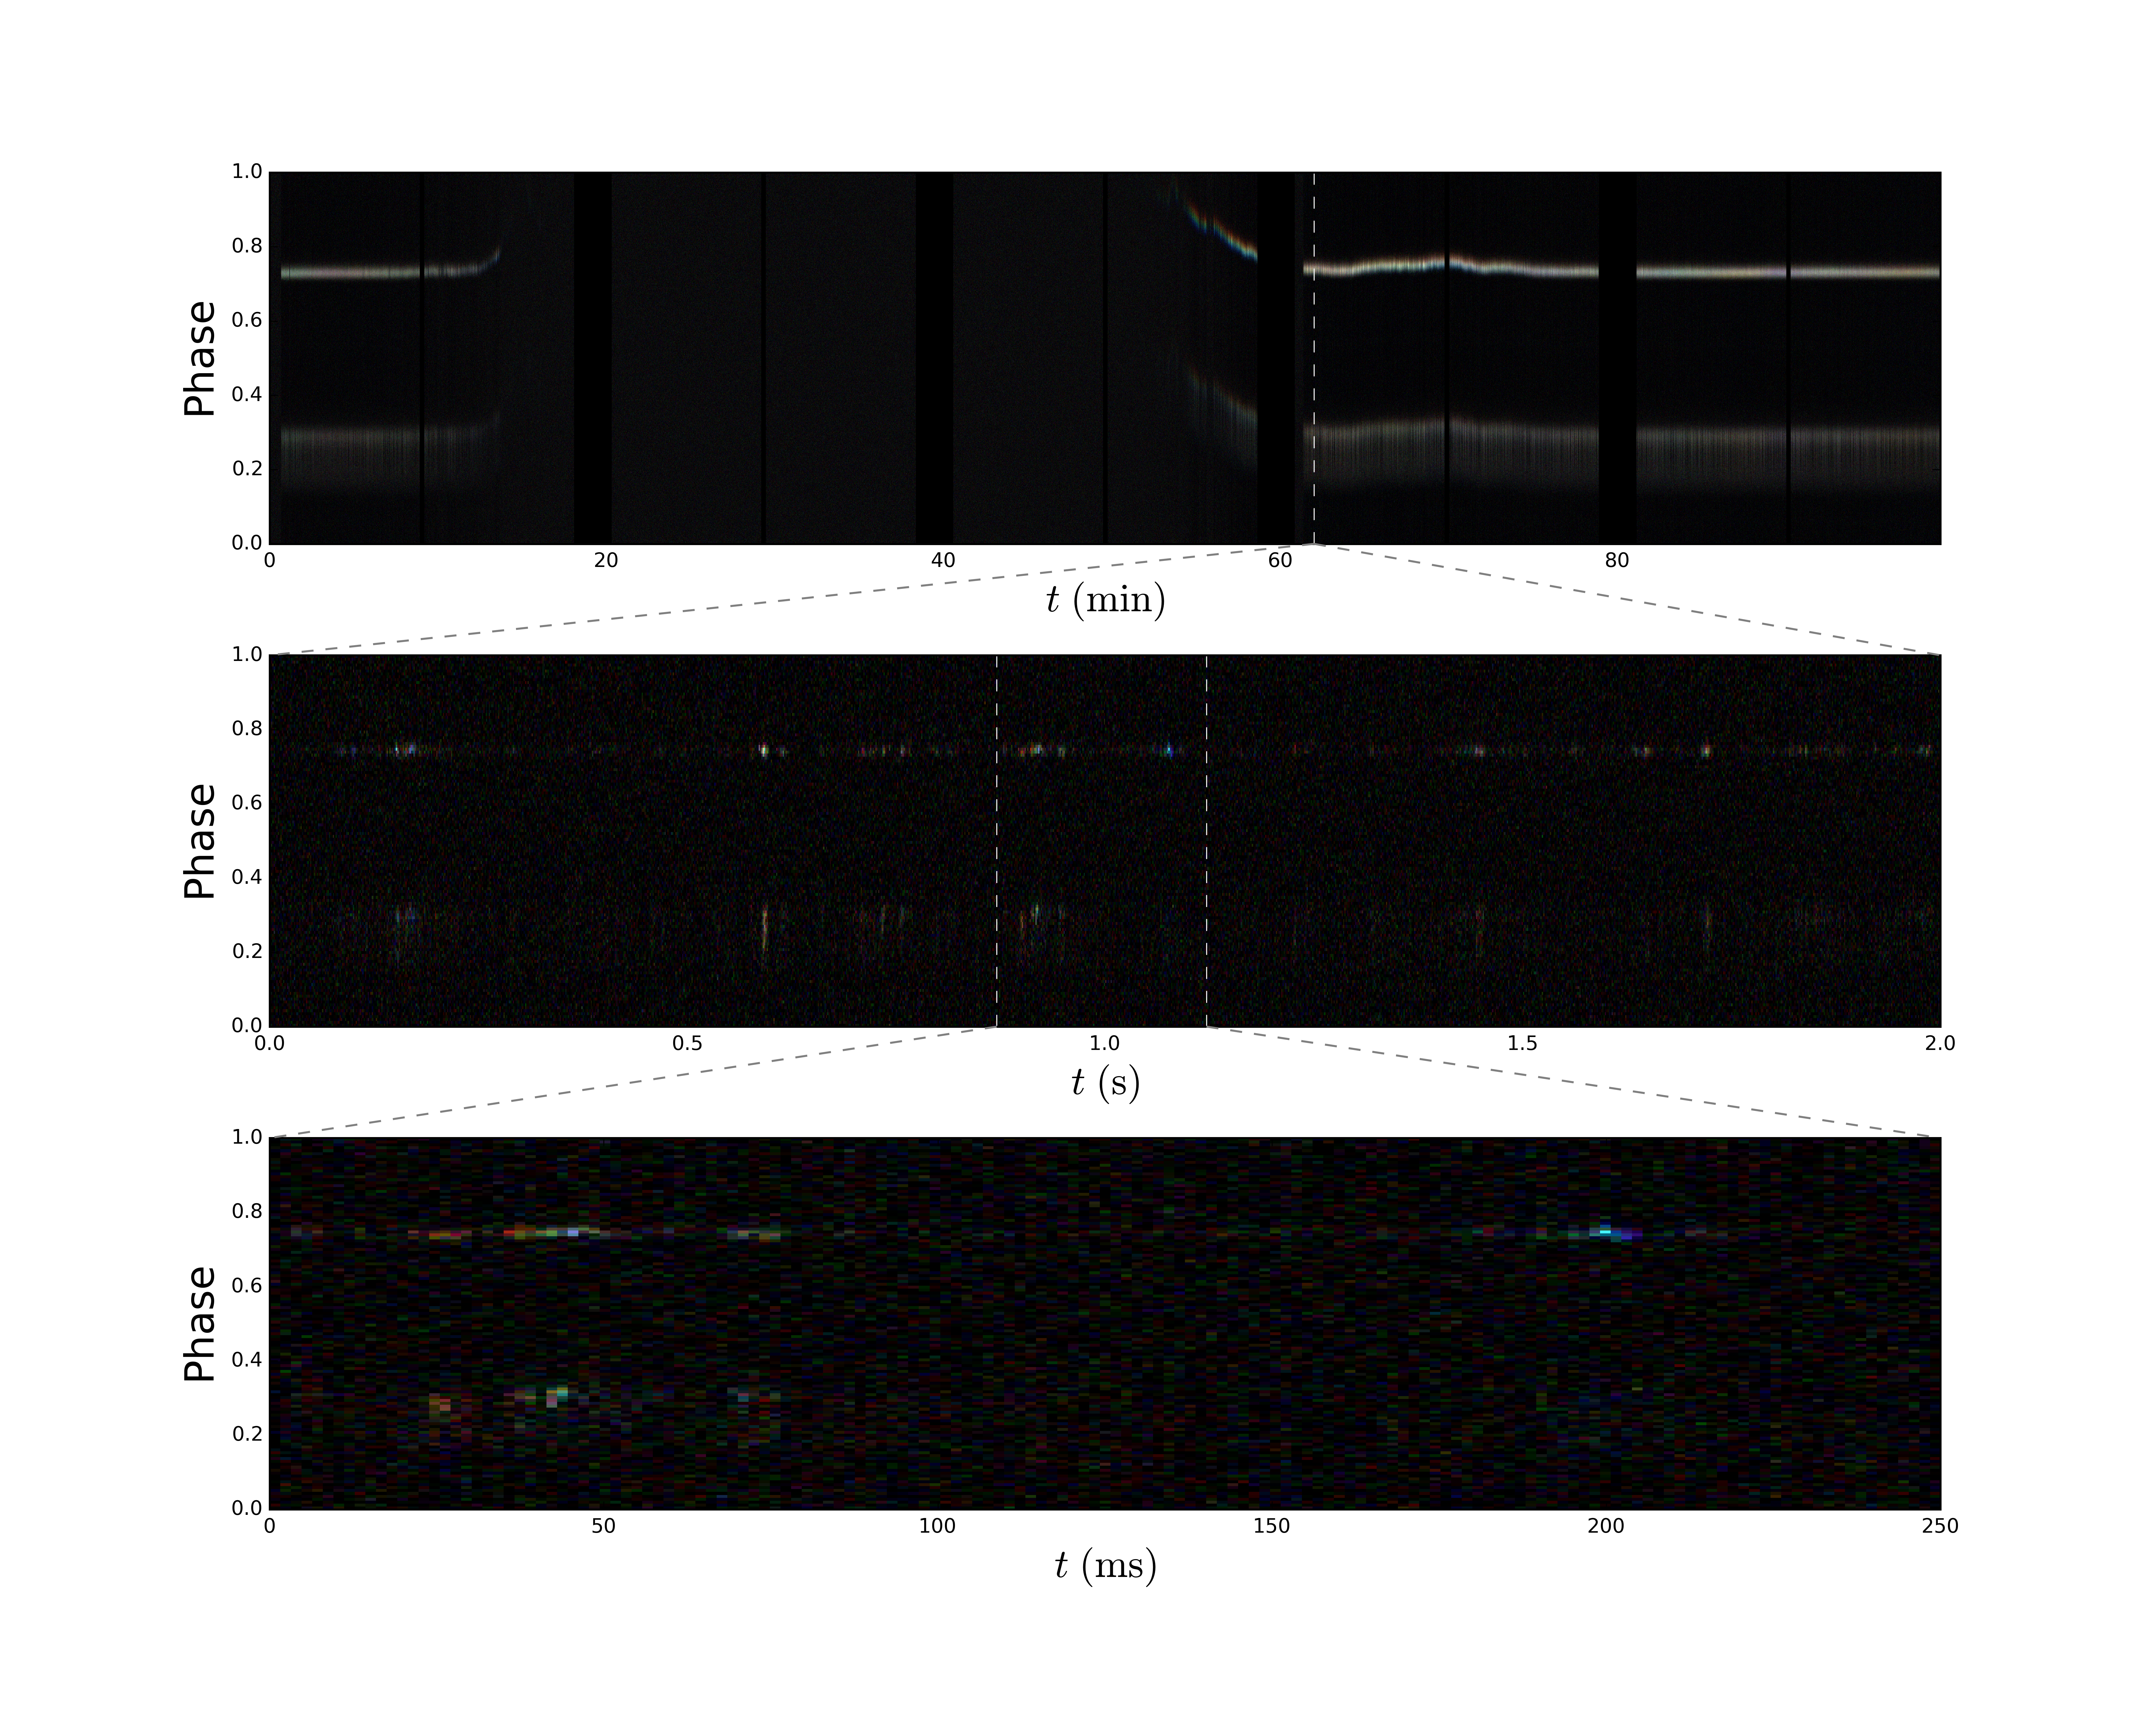
\includegraphics[width=0.8\textwidth]{Figures/LensingPanel-Landscape.png}

(Main et al 2017 in prep)
}
\frame{
    \frametitle{Lensing}
\includegraphics[width=2.5\textwidth]{Figures/LensingPanel3.png}
}
  \frame{
    \frametitle{Questions resolved}
    \begin{itemize}
    \item scattering not intervening galaxy or IGM: FRB110523 (Masui et al 2015)
    \item some FRBs repeat
     \item VLBI holds key
    \end{itemize}
  }

  \frame{
    \frametitle{Questions confused}
    \begin{itemize}
    \item Euclidean/spatial distribution?
    \item caveat: Bayesian arguments, look elsewhere effect, etc.
    \item repetition statistics?
    \item error underestimates?
    \end{itemize}
  }

  \frame{
    \frametitle{Repetition}
    \begin{itemize}
    \item Opperman et al arXiv:1705.04881
      \item Weibull: single parameter clustered generalization of Poisson statistics.
      \item statistics of independent intervals.
      \item $\xi \propto t^{-0.66}$ is $10^{12}$ times more likely
        than Poisson
        \item repeat rate $5.5$/day, non-poisson suggests rate is
          consistent with ALL FRB non-repetition for same rate!
    \end{itemize}
  }

\frame{
    \frametitle{non-Poisson}
     \includegraphics[width=1.0\textwidth]{Figures/n_singleint.pdf}

(Oppermann \& UP)
}

\section{FRBs}


\frame{
    \frametitle{FRB110523}
     \includegraphics[width=0.8\textwidth]{Figures/nature15769-f1.jpg}

Masui et al 2015
}


\frame{
    \frametitle{Scattering}
     \includegraphics[width=1.1\textwidth]{Figures/TwoScreenGeometry.png}
(figure credit: R. Main)
}

  \frame{
    \frametitle{Two screen physics}
    \begin{itemize}
      \item FRB110523:
      \item long $\sim 1$ms: local to host
      \item short $\sim 1 \mu$s: galactic (off plane)
      \item FRB121102:
      \item short $\sim 10$ns: local to host
      \item long $\sim 20 \mu$s: galactic (in plane)
    \end{itemize}
  }
  \frame{
    \frametitle{Depolarization}
    \begin{itemize}
    \item of all known radio magnetars, 1 in 4(?) has $|RM|>60,000$
    \item depolarized below 3GHz due to multipath propagation (near
      source)
    \item if seen from outside galaxy, probably still high RM and
      depolarization, but little scattering.
    \item store baseband data!
    \end{itemize}
  }

\section{Summary}

  \frame{
    \frametitle{Conclusion}
    \begin{itemize}
      \item FRB121102: binary plasma lensing?  up to 100x observed for PSRB1957+20
      \item ISM structure: mapping cosmic plasma and magnetic fields
      \item potentially already constrains Lorenz boosted models for FRB121102
      \item galactic centre magnetar (and maybe crab) important example for
        understanding FRBs
      \item propagation may affect (de-) polarization, high RM
        possible, save baseband data!
        \item caveats: always beware of statistics!
      \item future possibilities: CGM, IGM, localization, DM$(z)$ cosmology?

    \end{itemize}
  }

\end{document}
